\documentclass[a4paper,10pt]{article}
\usepackage{fullpage}
\usepackage{float}
\usepackage[english]{babel}
\usepackage{graphicx,subfig,wrapfig}
\usepackage{amsmath,amsfonts,amsthm,amssymb}
\usepackage{fancyhdr,fancybox,color}
\usepackage{enumerate}
\usepackage[amssymb]{SIunits}
\definecolor{MyBlue}{rgb}{0,0.3,0.6}
\usepackage[colorlinks=true,
            linkcolor=MyBlue,
            plainpages=false,
            citecolor=MyBlue,
            urlcolor=MyBlue]{hyperref}
\usepackage[all]{hypcap}
\usepackage[url=false,
backend=bibtex,
style=authoryear-comp,
doi=true,
isbn=true,
backref=false,
dashed=false,
maxcitenames=2,
maxbibnames=99,
natbib=true]{biblatex}
\DeclareNameAlias{author}{last-first}
\renewbibmacro{in:}{}

\addbibresource{reference.bib}
\nonfrenchspacing

\begin{document}
\noindent Chair: Physics of Fluids group
\begin{center}
 \begin{LARGE}
  Drops and bubbles spreading on lubricant infused surfaces
 \end{LARGE}
\end{center}

\section*{Description}

The spreading of liquid drops and air bubbles on solid surfaces is a complex phenomenon with various natural and industrial applications. Recently, a new class of surfaces, called liquid infused surfaces (LIS), has been developed that allows for unprecedented control over the spreading behavior of liquids and gases on solid surfaces. In this proposal, we aim to investigate the spreading behavior of liquid drops and air bubbles on LIS and explore its potential applications in different fields. 

Figure~\ref{Figure::Typical} illustrates a typical scenario when an air bubble in water comes in contact with LIS. Due to change in topology at the point of contact, a train of capillary waves travel across the bubble-water interface (figure~\ref{Figure::Typical}a,b,c). These traveling capillary waves converge at the top of the bubble (figure~\ref{Figure::Typical}d,e) leading to entrainment of a smaller air bubble (figure~\ref{Figure::Typical}f,g). We will study this process in detail to understand the influence of various control parameters on this spreading dynamics. 

\begin{figure}[H]
	\begin{center}
		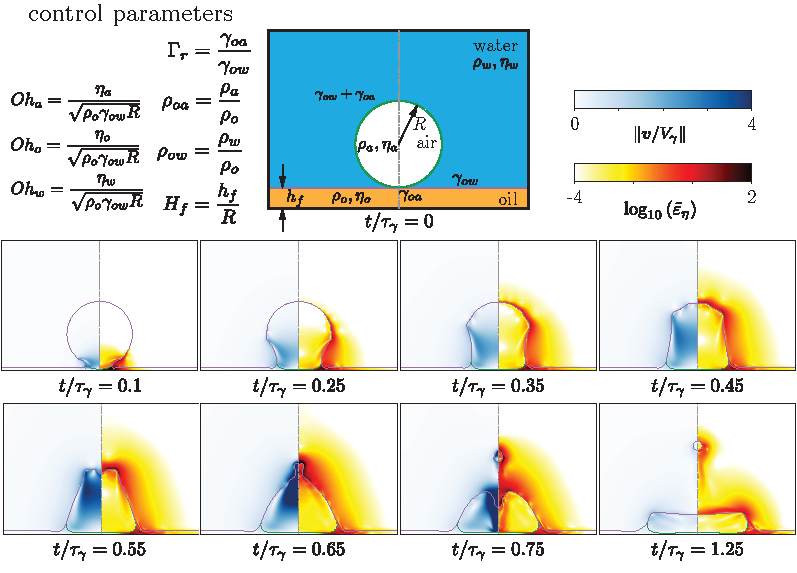
\includegraphics[width=0.95\textwidth]{BubbleOnLIS.pdf}
		\caption{A typical scenario of an air bubble in water spreading on liquid infused surfaces (LIS). In each snapshot, left-hand side contains information about the velocity field magnitude normalized with the inertio-capillary velocity and the right-hand side shows viscous dissipation function ($\varepsilon_\eta = 2\eta\left(\boldsymbol{\mathcal{D}:\mathcal{D}}\right)$). The latter is plotted on a $\log$ scale to identify regions of high viscous dissipation. Also see the video of this process at: \href{https://www.youtube.com/watch?v=crRoP9udk9M}{https://www.youtube.com/watch?v=crRoP9udk9M}.}
		\label{Figure::Typical}
\end{center}
\end{figure}

\noindent The main objectives of this study are:

\begin{enumerate}
	\item To investigate the spreading behavior of liquid drops and air bubbles on LIS under different conditions, such as liquid and geometric properties (see figure~\ref{Figure::Typical}). 
	\item To understand the underlying mechanisms that govern the spreading behavior of liquid drops and air bubbles on LIS. 
	\item To identify and explore the different timescales relevant for this process (see the introduction of \citet{VatsalThesis}).
\end{enumerate}

\section*{What will you do and what will you learn?}
In the Physics of Fluids group, we are looking for enthusiastic students to work on this topic.
\begin{enumerate}
\itemsep0em
\item You will learn about fundamental fluid dynamics.
\item You will get hands-on experience with Computational Fluid Dynamics (CFD).
\item You will learn how to do basic and advanced data analysis.
\item You will learn modeling of complex multiphase systems contact lines. 
\item You will learn how to document and publish ready-to-use codes and share them with the community, similar to \citet{basiliskVatsal, basiliskVatsalDropFilm, basiliskVatsalViscousBouncing}. 
\end{enumerate}

If you have any questions, fell free to contact \href{mailto:vatsalsanjay@gmail.com}{Vatsal} (details below).
\begin{center}
\begin{tabular}{|l|l|l|}
\hline \textbf{Supervision} & \textbf{E-mail} & \textbf{Office} \\
\hline Dr. Vatsal Sanjay & \href{mailto:vatsalsanjay@gmail.com}{vatsalsanjay@gmail.com} & Meander 246B \\
\hline Dr. Alexandros Oratis   & \href{mailto:a.t.oratis@utwente.nl}{a.t.oratis@utwente.nl}& Meander 250 \\
\hline Prof. Dr. Detlef Lohse & \href{mailto:d.lohse@utwente.nl}{d.lohse@utwente.nl} & Meander 261  \\
\hline
\end{tabular}
\end{center}

\printbibliography

\end{document}
